% Appendix Template

\chapter{Base de dades de l'Orchestrator} % Main appendix title

\label{OrchestratorDB} % Change X to a consecutive letter; for referencing this appendix elsewhere, use \ref{AppendixX}

Disseny i implementació de la base de dades del component \textit{Orchestrator}, d'acord amb els criteris establerts pel projecte SUPERSEDE. Per aquesta, s'ha decidit fer un disseny que garanteixi l'emmagatzemament de l'\textbf{historial de la base de dades} (duplicant les taules per mantenir totes les modificaicons realitzades). Per altra banda, les configuracions s'han materialitzat aplicant la tècnica de \textit{Single Table Inheritance}, i per tant no es distingeix entre tipus de configuracions (aquelles que no defineixin un atribut, tenen per valor per defecte \textit{null}).\\

Podeu consultar l'esquema a la següent pàgina.

\begin{figure}[!h]
\centering
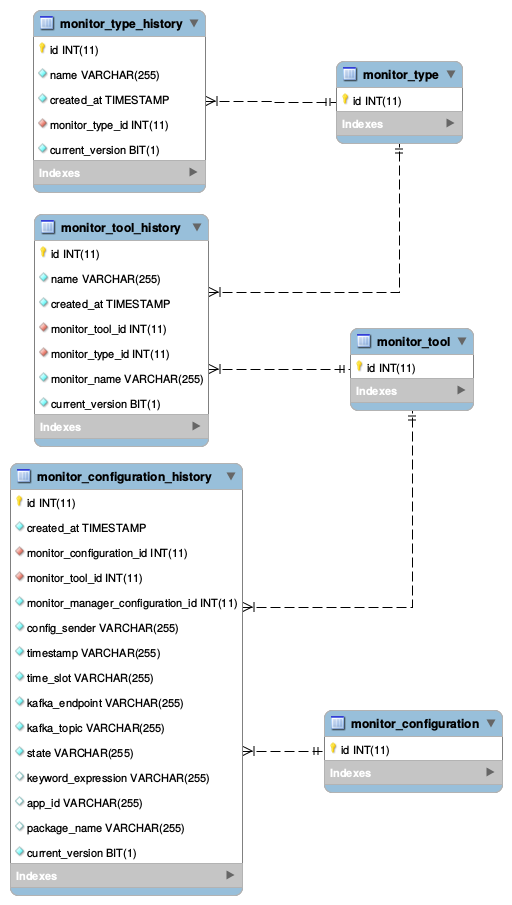
\includegraphics[width=12cm]{Figures/orchestratordb}
\decoRule
\caption{Disseny de la base de dades de l'Orchestrator}
\label{fig:orchestratordb}
\end{figure}